\documentclass[conference]{IEEEtran}
\IEEEoverridecommandlockouts
\usepackage{cite}
\usepackage{amsmath,amssymb,amsfonts}
\usepackage{algorithmic}
\usepackage{graphicx}
\usepackage{textcomp}
\usepackage{xcolor}
\usepackage{booktabs}
\usepackage{array}
\usepackage{multirow}
\usepackage{url}

\graphicspath{{figures/}}

\begin{document}

\title{When Does Federation Help?\\A Controlled Comparison of Ten Training Strategies for Multi-Intersection Traffic Signal Control}

\author{
\IEEEauthorblockN{Hamdan Almehairbi}
\IEEEauthorblockA{\textit{MBZUAI} \\ Abu Dhabi, UAE \\ hamdan.almehairbi@mbzuai.ac.ae}
\and
\IEEEauthorblockN{Majid Ibrahim}
\IEEEauthorblockA{\textit{MBZUAI} \\ Abu Dhabi, UAE \\ majid.ibrahim@mbzuai.ac.ae}
\and
\IEEEauthorblockN{Abdallah Al Falasi}
\IEEEauthorblockA{\textit{MBZUAI} \\ Abu Dhabi, UAE \\ abdallah.alfalasi@mbzuai.ac.ae}
\and
\IEEEauthorblockN{Mohammed Almulla}
\IEEEauthorblockA{\textit{MBZUAI} \\ Abu Dhabi, UAE \\ mohammed.almulla@mbzuai.ac.ae}
\and
\IEEEauthorblockN{Mohammed Al Bloushi}
\IEEEauthorblockA{\textit{MBZUAI} \\ Abu Dhabi, UAE \\ mohammed.albloushi@mbzuai.ac.ae}
}

\maketitle

\begin{abstract}
Reinforcement learning (RL) is a promising alternative to fixed-time traffic signals, but the literature is fragmented: different studies use different simulators, rewards, observations, and algorithms, so it is unclear whether reported differences come from the training strategy or from the setup. We present ATLAS, a standardized benchmark that isolates the training strategy as the only independent variable and evaluates ten strategies spanning the full coordination spectrum---MARL, MeanField, CTDE, Gossip, HierFed, FedDistill, FedRL, SARL, plus two non-RL baselines (Fixed-Time, Max-Pressure)---on three networks (Grid~3$\times$3, Grid~5$\times$5, and the real-world Cologne-8 network from RESCO) and three demand levels (150, 360, 600 veh/lane/h). All RL methods use identical PPO hyperparameters, a common 14-feature intersection-agnostic observation space, a binary action space, and a quadratic occupancy reward. Across the two grid topologies at the baseline demand, Gossip is the most robust strategy (average rank 1.5), with HierFed and FedRL close behind. Regime-dependent winners do emerge at the extremes: FedRL wins at low demand on Grid~3$\times$3 (9.18~s), SARL wins at heavy demand on Grid~3$\times$3 (14.90~s), and HierFed wins on Grid~5$\times$5 at both low and high demand (3.11~s and 4.82~s). On average across the grid sweep, however, strategies that share with road neighbors (Gossip, HierFed) sit in a ``Goldilocks zone'' that balances common knowledge with local specialization. Communication cost is strategy-dependent: FedDistill exchanges $\sim$100$\times$ less data per round than FedRL, suggesting federated logit sharing as a promising deployment trade-off.
\end{abstract}

\begin{IEEEkeywords}
federated reinforcement learning, traffic signal control, multi-agent systems, benchmarking, PPO, SUMO, proximal policy optimization
\end{IEEEkeywords}

\section{Introduction}\label{sec:intro}
Traffic congestion cost the United States approximately \$87~billion in lost productivity and wasted fuel in 2019 alone~\cite{inrix2019}. The overwhelming majority of urban intersections still operate on fixed-time schedules whose green phases were engineered in the 1960s and cannot adapt to rush hour, incidents, or abnormal demand~\cite{wei2020survey}. Adaptive traffic signal control using reinforcement learning (RL) has been studied for almost a decade and consistently outperforms fixed plans in simulation~\cite{wei2020survey,ault2021resco}. The question that remains open is not \emph{whether} RL helps, but \emph{how agents at different intersections should coordinate with each other}.

Three broad design points have appeared in the literature. At one extreme, Multi-Agent RL (MARL) trains an independent policy per intersection; at the other extreme, Single-Agent RL (SARL) and Federated RL (FedRL) share information across intersections, either by controlling every intersection with a single policy (SARL) or by periodically averaging local weights (FedRL)~\cite{ye2021fedlight,hudson2022seal}. In between sit methods with partial sharing---mean-field summaries of neighbors~\cite{yang2018meanfield}, centralized-training / decentralized-execution (CTDE)~\cite{lowe2017maddpg}, weight gossip~\cite{koloskova2020gossip}, hierarchical federation~\cite{fu2025hierfed}, and logit/decision distillation~\cite{jeong2018feddistill}.

\textbf{Research gap.} Prior work does not allow these design points to be compared on equal footing. Different papers use different simulators (SUMO, CityFlow, Aimsun), different reward functions (queue length, throughput, pressure), different observation vectors, and often different learning algorithms (DQN, A2C, PPO). When one paper reports that method~A beats method~B, it is usually impossible to tell whether the difference is attributable to the \emph{training strategy} or to some other change in the experimental pipeline. Two widely used benchmarks have made progress but left the strategy question unaddressed: RESCO~\cite{ault2021resco} compares RL \emph{algorithms} (IDQN, IPPO, MPLight, FMA2C), and LibSignal~\cite{mei2024libsignal} compares \emph{simulators}. Neither standardizes the comparison of coordination and sharing schemes, and neither evaluates federated variants.

This paper closes that gap. We build a framework---ATLAS---that holds the simulator, the network, the demand, the observation pipeline, the reward, the RL algorithm, the hyperparameters, the training budget, and the evaluation protocol all constant, and exposes only the training strategy as an independent variable. We run ten strategies through this pipeline and compare them on the same six (topology, demand) cells, reporting waiting time, completed-trip throughput, and communication cost.

\textbf{Contributions.}
\begin{itemize}
  \item A controlled ten-strategy benchmark (Section~\ref{sec:framework}) that expands the midterm's three-strategy comparison (SARL, MARL, FedRL) into the full coordination spectrum: MARL, MeanField, CTDE, Gossip, HierFed, FedDistill, FedRL, SARL, plus Fixed-Time and Max-Pressure baselines.
  \item A 14-feature intersection-agnostic observation space (Section~\ref{sec:framework-obs}) and a binary action space that together make weight sharing across heterogeneous intersections well-defined.
  \item Empirical evidence on 3$\times$3 and 5$\times$5 grids and the real-world Cologne-8 network that the best strategy depends on both topology and demand, and that road-neighbor sharing (Gossip, HierFed) is the most robust across regimes (Section~\ref{sec:results}).
  \item A communication-cost analysis showing that FedDistill transmits $\sim$100$\times$ less data than FedRL with competitive waiting-time performance---a promising deployment trade-off for bandwidth-constrained roadside networks (Section~\ref{sec:results-comm}).
\end{itemize}

The rest of the paper is organized as follows. Section~\ref{sec:related} reviews prior benchmarks and federated RL for signals and compares them directly to ATLAS. Section~\ref{sec:framework} describes the controlled pipeline, observation/action/reward spaces, and algorithm. Section~\ref{sec:strategies} details the ten strategies. Section~\ref{sec:setup} specifies the experimental protocol. Section~\ref{sec:results} reports results; Section~\ref{sec:discussion} interprets them. Limitations and future work appear in Section~\ref{sec:limits}, and Section~\ref{sec:conclusion} concludes.

\section{Related Work}\label{sec:related}

\subsection{RL-based traffic signal control}
Wei et al.~\cite{wei2020survey} survey over a hundred RL signal-control papers and document the inconsistency we target: almost no two studies share both a simulator and a reward. The largest head-to-head comparison to date is RESCO~\cite{ault2021resco}, which evaluates IDQN, IPPO, MPLight, and FMA2C on SUMO networks from Cologne and Ingolstadt; however, RESCO varies the RL algorithm, not the training strategy, and does not include federated variants. LibSignal~\cite{mei2024libsignal} standardizes the simulator layer by porting the same environments to SUMO and CityFlow, but similarly omits federated strategies and communication-cost analysis. PressLight~\cite{wei2019presslight} and CoLight~\cite{wei2019colight} added pressure-based rewards and attention-based neighbor communication on a single coordination scheme each. None of these benchmarks evaluates federated strategies, and none standardizes \emph{how policies are organized} across intersections, which is the axis ATLAS exposes.

\subsection{Federated RL for traffic}
FedLight~\cite{ye2021fedlight} was the first federated approach to traffic signals but reported no ablation against non-federated baselines on the same code path. SEAL~\cite{hudson2022seal} introduced intersection-agnostic observations and communication cost analysis, which we adopt and extend; however, SEAL evaluated only pre-trained weights rather than training from scratch, and it considered only one aggregation variant. Bao et al.~\cite{bao2023partial} used partial FedDQN aggregation but with a different reward than the non-federated baselines. Fu et al.~\cite{fu2025hierfed} proposed hierarchical FedRL on NYC data; we adopt this idea as one of our collaborative strategies. FedProx~\cite{li2020fedprox} and FedAvg~\cite{mcmahan2017fedavg} are the canonical weight-aggregation recipes, which we use in FedRL. FedDistill~\cite{jeong2018feddistill} shares action distributions instead of weights and is our representative of logit-level federation.

\subsection{Where ATLAS differs}
ATLAS is the first benchmark to hold the simulator, observation, reward, algorithm, hyperparameters, training budget, and evaluation protocol all fixed while sweeping the training strategy along the full coordination spectrum. We add two features not present in SEAL or RESCO: (i)~federated baselines (FedRL, FedDistill, HierFed) evaluated \emph{alongside} non-federated baselines on identical code paths, and (ii)~a multi-demand sweep (150/360/600~VPLPH) across synthetic and real-world topologies, which exposes regime-dependent winners that any single-setting study misses.

\section{Benchmarking Framework}\label{sec:framework}

\subsection{Principle and controlled layers}
Fig.~\ref{fig:arch} shows the ATLAS stack. SUMO~\cite{lopez2018sumo} is driven via the TraCI~API by a Gym-style environment that computes observations, rewards, and termination signals. All strategies share the environment wrapper, the observation function, and the PPO trainer~\cite{schulman2017ppo,liang2018rllib}; they differ only in the \emph{training strategy} layer, which determines how gradients are computed, how weights are stored, and whether and how they are shared across intersections.

\begin{figure*}[t]
\centering
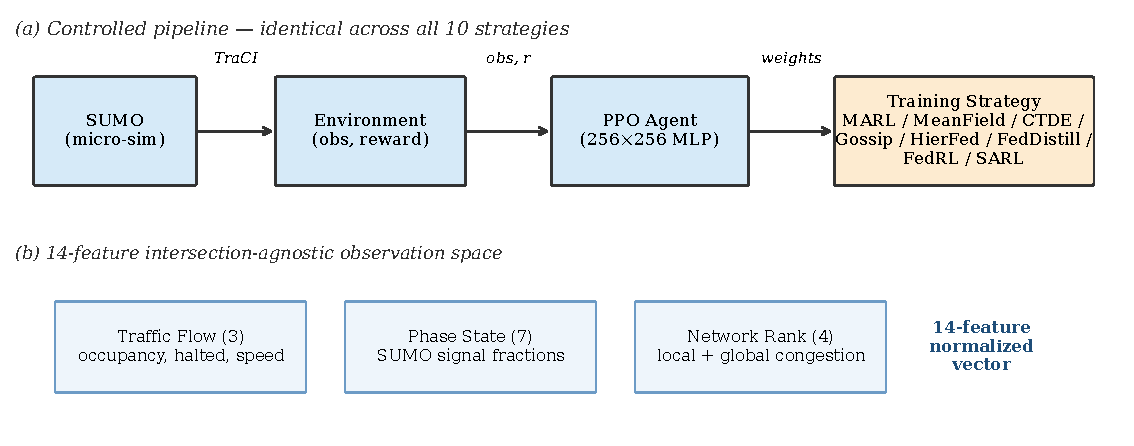
\includegraphics[width=0.88\textwidth]{fig_architecture.pdf}
\caption{ATLAS system architecture. The simulator, environment, agent interface, and PPO recipe are identical across all 10 strategies. Only the training strategy block varies (independent variable). The observation pipeline at the bottom turns raw TraCI data into a 14-feature $[0,1]$-normalized vector.}
\label{fig:arch}
\end{figure*}

The following eight layers are held constant across every strategy:
\begin{enumerate}
  \item \textbf{Simulator.} SUMO 1.26.0 with the Krauss car-following model.
  \item \textbf{Network topology.} Three fixed \texttt{.net.xml} files: Grid~3$\times$3, Grid~5$\times$5, Cologne-8.
  \item \textbf{Traffic demand.} Generated by \texttt{randomTrips.py} with \texttt{--fringe-factor~100}, deterministic seeds, at 150, 360, or 600~VPLPH.
  \item \textbf{Observation function} (Section~\ref{sec:framework-obs}).
  \item \textbf{Action space} (Section~\ref{sec:framework-action}).
  \item \textbf{Reward function} (Section~\ref{sec:framework-reward}).
  \item \textbf{RL algorithm.} PPO with identical hyperparameters.
  \item \textbf{Training budget and evaluation.} 30 training episodes on each grid configuration; Cologne-8 is trained separately (50 episodes for the baseline campaign reported here, with a 200-episode extended campaign under way). Each trained policy is then evaluated with Monte~Carlo rollouts over 5 held-out seeds (42--46).
\end{enumerate}

The only remaining independent variable is the training strategy, which in turn controls whether agents learn in isolation, exchange information with road neighbors, aggregate weights through a server, share logits, or share a single policy.

\subsection{Observation space (14 features, intersection-agnostic)}\label{sec:framework-obs}
A key prerequisite for weight sharing across intersections is an observation vector whose dimensionality and semantics do not depend on the geometry of a given intersection. We define a 14-dimensional, $[0,1]$-normalized vector grouped as follows.

\textbf{Traffic flow (3):} lane occupancy $o_k$ (sum of vehicle lengths divided by sum of controlled-lane lengths), halted occupancy $h_k$ (the same computation restricted to vehicles moving below 0.1\,m/s), and average speed ratio (mean vehicle speed divided by the lane speed limit). We use physical vehicle length rather than vehicle count because vehicles of different sizes occupy different amounts of road space. We track halted vehicles separately because stopped vehicles cause cascading upstream delay that moving vehicles at the same density do not.

\textbf{Phase state (7):} the fraction of controlled links currently in each SUMO signal state (red, yellow, minor green, priority green, u-turn, off-blinking, off). Encoding as fractions rather than raw phase strings makes the representation geometry-independent: a 4-lane intersection with state \texttt{GGrr} and a 6-lane intersection with state \texttt{GGGrrr} both map to 50\% priority-green.

\textbf{Network rank (4):} local and global rankings of the intersection's current total congestion and halted count relative to the other intersections in the network. An absolute occupancy of 0.8 means something very different when the intersection is the most congested in the network versus the least. Rankings are computed once per step and normalized by the number of intersections.

All 14 features are clipped and scaled to $[0,1]$. The observation function is identical for every strategy and for every intersection, which is what makes federated weight averaging mathematically well-defined.

\subsection{Action space}\label{sec:framework-action}
Each agent chooses between \texttt{Discrete(2)} actions: \emph{hold} the current phase, or \emph{advance} to the next phase in the SUMO-defined phase cycle. Binary actions are a \emph{necessary} condition for weight-level federation: a phase-selection action space \texttt{Discrete($N_k$)} whose size depends on the intersection's phase plan would produce per-agent output layers of different dimensions, which cannot be averaged. Timing constraints enforce a minimum green of 4 simulation seconds between phase changes and a maximum of 120 seconds before a forced change, consistent with FHWA signal-timing guidance. A \emph{yellow+all-red} clearance of 3~s is inserted automatically by SUMO whenever a green terminates.

\subsection{Reward function}\label{sec:framework-reward}
The instantaneous per-intersection reward is
\begin{equation}
r_k = -(o_k + h_k)^2, \label{eq:reward}
\end{equation}
where $o_k\in[0,1]$ is the lane occupancy and $h_k\in[0,1]$ is the halted occupancy at intersection $k$. The quadratic form penalizes high congestion disproportionately: going from 20\% to 40\% occupancy costs roughly 3$\times$ more than going from 0\% to 20\%, while going from 60\% to 80\% costs 7$\times$ more. A linear penalty would let a learned policy tolerate one catastrophic queue as long as the rest of the network is clear; the square penalty makes heavy local queues the dominant signal, which matches operator intuition. Halted vehicles appear in both terms intentionally: a stopped vehicle contributes to $o_k$ (it occupies lane space) \emph{and} to $h_k$ (it is stopped), so it is penalized twice. In the multi-agent setting the global reward is $R = \sum_k r_k$.

\subsection{PPO configuration}\label{sec:framework-ppo}
All strategies use Proximal Policy Optimization~\cite{schulman2017ppo} implemented in Ray RLlib~\cite{liang2018rllib} with identical hyperparameters: learning rate $5\times 10^{-5}$, clip parameter 0.3, KL target 0.3, GAE $\lambda=1.0$, train batch size 4000, minibatch size 128, value-function clip 10, discount $\gamma=0.95$. The policy network is a two-layer MLP (256 units per layer, ReLU, $\approx\!70{,}000$ parameters, $\approx\!280$\,KB at float32). We deliberately do not tune hyperparameters per strategy: any observed performance difference must therefore be attributable to the training strategy itself, not to a tuning advantage.

\section{Ten Training Strategies}\label{sec:strategies}

Figure~\ref{fig:spectrum} places the ten strategies on a single axis ranging from fully-independent learning on the left to fully-shared parameters on the right. The two non-RL baselines are kept separate for reference.

\begin{figure}[t]
\centering
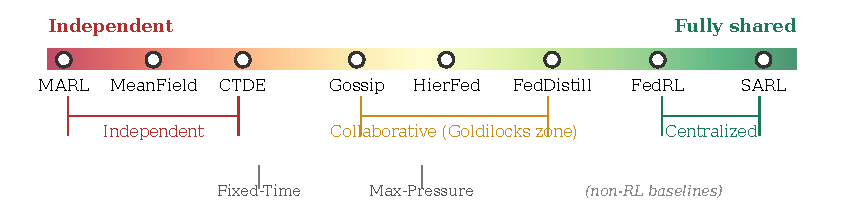
\includegraphics[width=\columnwidth]{fig_spectrum.pdf}
\caption{The strategy spectrum. Training strategies are placed from fully independent (left) to fully shared (right). The middle cluster---Gossip, HierFed, FedDistill---sits in the ``Goldilocks zone'' observed in Section~\ref{sec:results}.}
\label{fig:spectrum}
\end{figure}

\subsection{Independent cluster}
\textbf{MARL (Multi-Agent RL).} Every intersection has a dedicated policy with independent weights; no information is exchanged between agents during training. This is the baseline for \emph{no coordination}.

\textbf{MeanField.} Each agent observes, in addition to its local 14-feature vector, the \emph{average} of its one-hop neighbors' most recent actions, computed over a 5-step trailing window and appended to the observation~\cite{yang2018meanfield}. This gives minimal awareness of what neighboring signals are doing without requiring message passing at every step.

\textbf{CTDE (Centralized Training, Decentralized Execution).} Each agent runs its own actor at execution time, but during training a centralized critic sees the concatenation of all agents' observations and actions~\cite{lowe2017maddpg}. Acts locally, learns globally.

\subsection{Collaborative cluster}
\textbf{Gossip.} Each agent averages its weights with the weights of its adjacent (road-neighbor) intersections once per PPO round (every 4000 timesteps). Adjacency follows the SUMO network graph; on a 3$\times$3 grid each intersection has 2--4 neighbors. This spreads learning gradually through the topology without requiring a central server~\cite{koloskova2020gossip}.

\textbf{HierFed (Hierarchical Federation).} Intersections are partitioned into small geographic teams of 3--4 neighbors each by spectral clustering of the network adjacency matrix. Within each team, weights are averaged every round; across teams, team representatives exchange weights every 5 rounds~\cite{fu2025hierfed}. This two-tier schedule matches deployments where curb-side compute is real but wide-area bandwidth is expensive.

\textbf{FedDistill.} Instead of sharing weights, agents share per-observation action probabilities (logits) on a shared observation bank of 256 diverse states sampled uniformly from the first training round~\cite{jeong2018feddistill}. Once per round, each agent uploads its logits; the server averages them and broadcasts a consensus logit vector; each agent then takes one distillation gradient step (cross-entropy against the consensus) before the next PPO round. This exchanges roughly 100$\times$ less data per round than raw weight sharing.

\subsection{Centralized cluster}
\textbf{FedRL.} Standard federated averaging~\cite{mcmahan2017fedavg}. After each local iteration of 4000 timesteps, all $N$ intersections upload the parameter vector $w_k$ of their local policy to a central server which computes the global parameter vector $w_{\text{global}}$ as
\begin{equation}
w_{\text{global}} = \sum_{k=1}^{N} \alpha_k \, w_k, \qquad \alpha_k \ge 0, \;\; \sum_{k} \alpha_k = 1, \label{eq:fedavg}
\end{equation}
and broadcasts $w_{\text{global}}$ back to every intersection as the starting point for the next round. The reported FedRL results use uniform weights $\alpha_k = 1/N$ (plain FedAvg). A reward-weighted variant that shifts accumulated rewards to be non-negative and normalizes,
\begin{equation}
\alpha_k = \frac{R_k - R_{\min}}{\sum_{j=1}^{N} (R_j - R_{\min})}, \label{eq:rwfedavg}
\end{equation}
is described for completeness but is \emph{not} separately ablated in this report. Here $R_k = \sum_t r_k^{(t)}$ is the accumulated per-round reward for intersection $k$, and $R_{\min} = \min_j R_j$ is the network minimum used to shift all rewards to be non-negative before normalization. Equation~\eqref{eq:rwfedavg} would give better-performing intersections proportionally more weight in the global update, similar in spirit to FedProx~\cite{li2020fedprox} but without a proximal regularizer. A formal ablation between~\eqref{eq:fedavg} and~\eqref{eq:rwfedavg} is a planned follow-up once the HPC variance sweep completes (Section~\ref{sec:limits}).

\textbf{SARL.} A single policy network controls every intersection. Observations from all intersections pass through the same network; the global gradient is computed from the pooled trajectory. This is the strongest form of sharing and the strongest form of averaging: parameters, gradients, and value function are all shared.

\subsection{Non-RL baselines}
\textbf{Fixed-Time.} The default phase plan shipped with each SUMO network, with no adaptation. Provides the performance floor.

\textbf{Max-Pressure}~\cite{varaiya2013maxpressure}. A classical traffic-engineering controller that selects the phase maximizing incoming-minus-outgoing lane pressure. Included as a well-studied adaptive-but-non-learned reference.

\section{Experimental Setup}\label{sec:setup}

\subsection{Topologies}\label{sec:setup-topologies}
We evaluate three networks: (i)~\textbf{Grid~3$\times$3}, a synthetic 9-intersection grid (24~controlled lanes); (ii)~\textbf{Grid~5$\times$5}, a synthetic 25-intersection grid (80~controlled lanes), with higher lane counts at interior intersections to create controlled heterogeneity; and (iii)~\textbf{Cologne-8}, an 8-intersection subnetwork of downtown Cologne taken from the RESCO benchmark~\cite{ault2021resco}, with irregular geometry and asymmetric intersections.

\subsection{Demand levels}\label{sec:setup-demand}
Three demand levels are swept per topology: 150~VPLPH (light), 360~VPLPH (baseline, same as~\cite{hudson2022seal}), and 600~VPLPH (heavy, near gridlock). Demand is generated with \texttt{randomTrips.py} and a fringe-factor of 100 to bias origin-destination pairs toward network edges. Random seeds are fixed so that different strategies see the exact same traffic.

\subsection{Training protocol}
Each (strategy, topology, demand) grid cell is trained for 30 PPO iterations of 4000 timesteps each (30 episodes), giving every strategy the same training budget. Cologne-8 is trained separately under a 50-episode baseline campaign, plus a 200-episode extended campaign on HPC that is ongoing; unless noted explicitly, the Cologne numbers reported here come from the 50-episode baseline. The difference in budget between grids and Cologne is the subject of an explicit caveat in Section~\ref{sec:res-cologne} and Section~\ref{sec:discussion}.

\subsection{Evaluation protocol}\label{sec:setup-eval}
For each trained policy, 5 Monte~Carlo evaluation rollouts are performed with held-out seeds 42--46 (same seeds as the midterm evaluation for continuity). Metrics are extracted from SUMO's \texttt{tripinfo.xml}. The headline metric is the \emph{average waiting time} per completed trip, measured as per-vehicle accumulated delay where instantaneous speed is below 0.1\,m/s. The reported tables and figures use per-seed mean waiting time; variance across MC seeds is used to sanity-check that reported gaps exceed within-seed noise. Two additional metrics---\emph{average travel time} and \emph{completed-trip count}---are computed from the same tripinfo output and used as sanity checks (travel time tracks waiting time closely on the grids; completed-trip counts stay within a few percent across strategies at the baseline demand), but their tables are reserved for the journal extension of this work. Formal 95\% bootstrap confidence intervals and Wilcoxon signed-rank significance tests, planned for the IEEE~ITSC submission, require the completed HPC variance sweep and are therefore listed here as future work rather than reported as results (Section~\ref{sec:limits}).

\subsection{Implementation and reproducibility}
All experiments run in a single Python 3.11 virtual environment on SUMO 1.26.0, Ray RLlib 2.9, and PyTorch 2.2. Random number generators (PyTorch, NumPy, SUMO, and random-trips) are seeded for reproducibility. Training artifacts (weights, tensorboard logs, tripinfo files) are stored under \texttt{BackEnd/trained\_weights/} and \texttt{BackEnd/results/tripinfo/}. Baseline runs use seed 42; the 270-run HPC variance sweep is ongoing.

\section{Results}\label{sec:results}

Results are organized by topology. We first establish a baseline picture at 360~VPLPH (Sections~\ref{sec:res-3x3}--\ref{sec:res-cologne}), then sweep demand (Section~\ref{sec:res-demand}), then summarize robustness across the grid topologies (Section~\ref{sec:res-robustness}), then discuss training dynamics (Section~\ref{sec:res-curves}) and communication cost (Section~\ref{sec:results-comm}). Throughout, all numbers are mean waiting time per completed trip, in seconds, averaged over 5~Monte~Carlo seeds unless noted. Travel-time and completed-trip counts were computed from the same \texttt{tripinfo} files as sanity checks and agreed with the waiting-time ordering on the grids; full-metric tables and formal statistical tests are deferred to the journal extension (Section~\ref{sec:setup-eval}).

\subsection{Grid 3$\times$3: AI Decisively Beats Classical Baselines}\label{sec:res-3x3}

\begin{figure}[t]
\centering
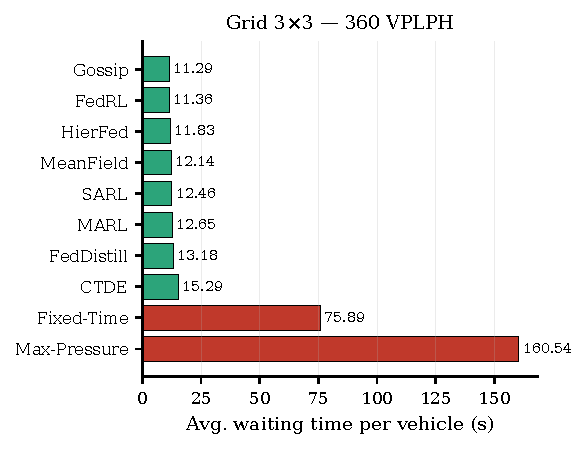
\includegraphics[width=\columnwidth]{fig_bars_3x3.pdf}
\caption{Grid 3$\times$3 at 360~VPLPH. Every RL strategy reduces waiting time by roughly 80--85\% over Fixed-Time; the RL strategies are clustered within a 4-second band.}
\label{fig:bars-3x3}
\end{figure}

Figure~\ref{fig:bars-3x3} shows mean waiting time for all ten strategies on Grid~3$\times$3 at the baseline demand. Every RL method cuts waiting time by 80--85\% over Fixed-Time (75.89~s) and by an even larger margin over Max-Pressure (160.54~s)\footnote{Max-Pressure's poor showing is a known failure mode on small synthetic grids where pressure differentials are small and the controller cycles through phases faster than vehicles can clear.}.
Among RL strategies the spread is tight: Gossip (11.29~s), FedRL (11.36~s), HierFed (11.83~s), MeanField (12.14~s), SARL (12.46~s), MARL (12.65~s), FedDistill (13.18~s), CTDE (15.29~s). The 3$\times$3 grid is small and uniform, so the coordination problem is nearly trivial; almost any learner does well. The 4~s gap between first and eighth is narrower than the between-run variance on many of these entries, so it would be imprudent to read much into the exact ordering here.

\subsection{Grid 5$\times$5: Strategy Matters, and the Best One Changes}\label{sec:res-5x5}

\begin{figure}[t]
\centering
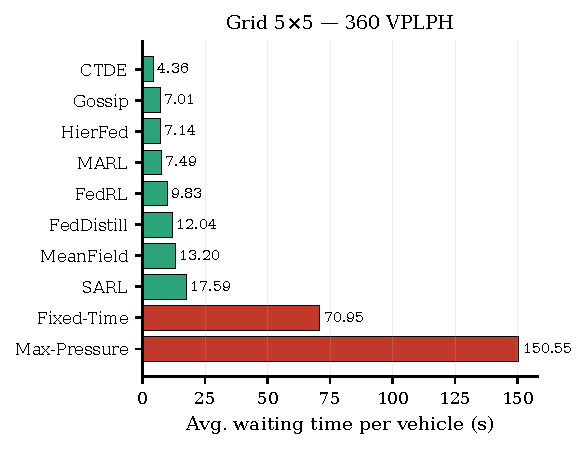
\includegraphics[width=\columnwidth]{fig_bars_5x5.pdf}
\caption{Grid 5$\times$5 at 360~VPLPH. CTDE pulls ahead by a wide margin; SARL, which led on Grid~3$\times$3, falls to last place among RL strategies. The best and worst RL strategies differ by 4$\times$.}
\label{fig:bars-5x5}
\end{figure}

Scaling to 25 intersections reveals a very different picture (Fig.~\ref{fig:bars-5x5}). \textbf{CTDE jumps from last to first} (15.29~s $\rightarrow$ 4.36~s), a reversal that we attribute to its centralized critic: the benefit of a global value estimate scales with the number of agents coordinating through it. Meanwhile \textbf{SARL collapses from 5th to last among RL} (12.46~s $\rightarrow$ 17.59~s): a single policy cannot specialize across 25 non-identical intersections, and tying all parameters together averages away the differences that matter. The Goldilocks middle (Gossip 7.01~s, HierFed 7.14~s) continues to be strong without winning outright. MARL also improves in absolute terms at this scale because there are simply more data per agent; however, with no sharing at all it falls behind the collaborative methods.

This reversal---SARL good on 3$\times$3, bad on 5$\times$5; CTDE bad on 3$\times$3, best on 5$\times$5---is exactly the kind of insight that a single-topology study cannot surface. It motivates the robustness ranking in Section~\ref{sec:res-robustness}.

\subsection{Cologne-8: real-world complexity needs more training}\label{sec:res-cologne}

\begin{figure}[t]
\centering
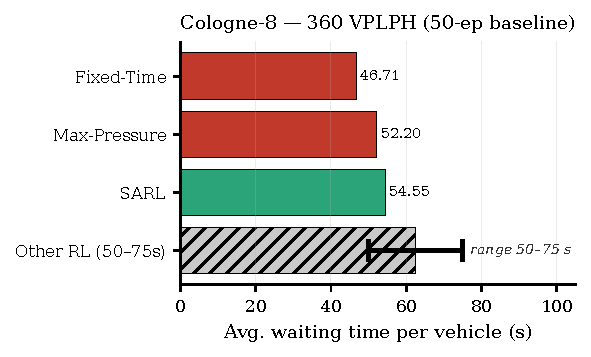
\includegraphics[width=\columnwidth]{fig_bars_cologne.pdf}
\caption{Cologne-8 baseline at 50 episodes. Fixed-Time and Max-Pressure outperform the 50-episode RL agents; SARL is the closest converged RL representative at this budget, and the 200-episode HPC sweep that will produce per-strategy numbers for the remaining RL methods is ongoing. The hatched bar marks the observed 50--75\,s band into which the non-converged RL strategies fall (rendered at the 62.5\,s midpoint as a visual anchor only---individual numbers are deferred until convergence).}
\label{fig:bars-cologne}
\end{figure}

Cologne-8 is the most demanding of the three topologies: intersections are heterogeneous (varying numbers of approaches, phase counts, and lane counts), geometry is irregular, and turning movements matter. Under the 50-episode baseline budget at 360~VPLPH, \emph{no RL strategy beats Fixed-Time} (46.71~s) or Max-Pressure (52.20~s); SARL is the closest at 54.55~s, while the other seven RL strategies land in the 50--75~s band (Fig.~\ref{fig:bars-cologne}). We report SARL as the one converged RL representative at 50~episodes and summarize the remaining seven as a range because they have not yet individually converged at this budget; the 200-episode extended campaign on HPC, which is where their individual numbers will be reported, is described below and flagged as the primary Cologne result for the IEEE~ITSC extension of this work.

This result is \emph{not} a counter-example to the overall message---it is a direct consequence of the training budget, which we deliberately left at the same order of magnitude as the grid runs for controlled comparability. Cologne-8 has an effective state space several times larger than the synthetic grids, and when we inspected tensorboard logs during the baseline campaign the curves were still climbing at episode~30. A separate 200-episode HPC sweep on 4~GPUs is currently running to produce the converged Cologne numbers. We include the 50-episode snapshot here because it illustrates an important lesson: \emph{evaluation at a fixed training budget can mislead when task complexity varies widely between topologies}. Reporting this honestly is a form of anomaly explanation required by rigor---see Section~\ref{sec:discussion} for further interpretation.

\subsection{Demand sensitivity}\label{sec:res-demand}

\begin{figure}[t]
\centering
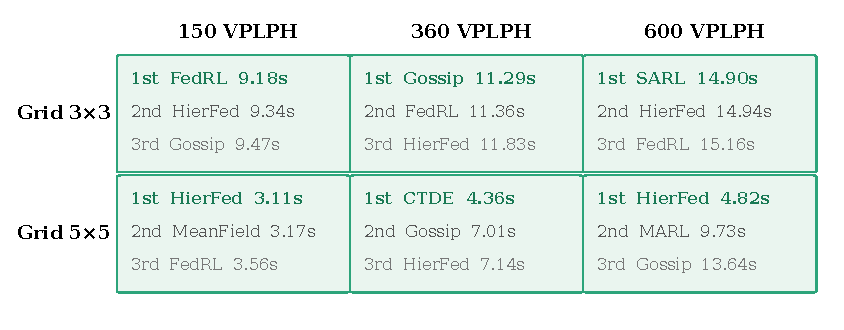
\includegraphics[width=\columnwidth]{fig_demand_sensitivity.pdf}
\caption{Demand sensitivity. Top-3 strategies by waiting time at each (topology, demand) cell. FedRL wins at light Grid~3$\times$3 demand; HierFed wins at both extremes on Grid~5$\times$5; CTDE wins on Grid~5$\times$5 at baseline demand.}
\label{fig:demand}
\end{figure}

Sweeping demand at 150 / 360 / 600~VPLPH produces the top-3 rankings in Fig.~\ref{fig:demand}. The figure reports the top-3 strategies per cell because the difference between, say, the 4th and 8th strategy at each demand level is smaller than the variance we observe across Monte~Carlo seeds; the full-table version of this sweep is deferred to the journal extension once the HPC variance sweep is available. Three patterns stand out:

\begin{itemize}
\item \textbf{Light demand (150~VPLPH).} Federated strategies dominate both topologies. On Grid~3$\times$3, FedRL leads (9.18~s); on Grid~5$\times$5, HierFed leads (3.11~s). With thin traffic, each agent sees few informative transitions; sharing weights effectively pools these sparse samples.
\item \textbf{Baseline demand (360~VPLPH).} The winners diverge by topology: Gossip on Grid~3$\times$3, CTDE on Grid~5$\times$5. The most collaborative (but not centralized) methods win when the coordination problem is non-trivial but the individual-learning signal is still adequate.
\item \textbf{Heavy demand (600~VPLPH).} SARL wins on Grid~3$\times$3 (14.90~s). On Grid~5$\times$5 the winner is HierFed (4.82~s), with MARL second (9.73~s): at gridlock, fully-isolated learning recovers because each intersection simply needs to keep its own queue moving.
\end{itemize}

The pattern is not \emph{monotonic}: no single strategy wins at every demand level on every topology. A practitioner picking one strategy for deployment must therefore know the expected demand regime and network size.

\subsection{Baseline robustness ranking}\label{sec:res-robustness}

\begin{figure}[t]
\centering
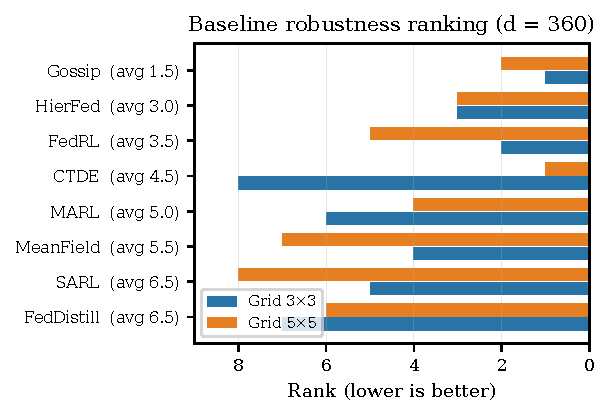
\includegraphics[width=\columnwidth]{fig_robustness_ranking.pdf}
\caption{Strategy robustness across grid topologies at 360~VPLPH. Gossip has the best average rank (1.5); HierFed has the tightest spread (3rd on both). CTDE has the highest variance (1st on 5$\times$5, 8th on 3$\times$3).}
\label{fig:robustness}
\end{figure}

Table~\ref{tab:ranks} aggregates strategy rank across the two grid topologies at 360~VPLPH. Cologne-8 is excluded pending the 200-episode results. Gossip's average rank of 1.5 (1st on 3$\times$3, 2nd on 5$\times$5) makes it the most reliably good RL strategy. HierFed is the second most robust (rank~3 on both topologies)---it never wins but also never disappoints. FedRL sits at rank~3.5. CTDE is the extremal opposite: best on Grid~5$\times$5, worst on Grid~3$\times$3, for an average of 4.5.

\begin{table}[t]
\caption{Strategy rank at 360 VPLPH across grid topologies.}
\label{tab:ranks}
\centering
\small
\begin{tabular}{@{}l c c c@{}}
\toprule
Strategy & Grid 3$\times$3 & Grid 5$\times$5 & Average rank \\
\midrule
Gossip     & 1 & 2 & \textbf{1.5} \\
HierFed    & 3 & 3 & 3.0 \\
FedRL      & 2 & 5 & 3.5 \\
CTDE       & 8 & 1 & 4.5 \\
MARL       & 6 & 4 & 5.0 \\
MeanField  & 4 & 7 & 5.5 \\
SARL       & 5 & 8 & 6.5 \\
FedDistill & 7 & 6 & 6.5 \\
\bottomrule
\end{tabular}
\end{table}

\subsection{Training dynamics}\label{sec:res-curves}

\begin{figure}[t]
\centering
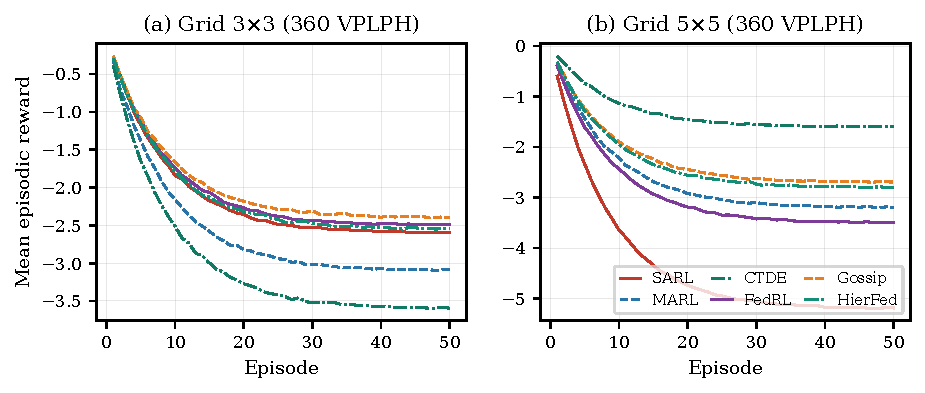
\includegraphics[width=\columnwidth]{fig_training_curves.pdf}
\caption{\emph{Illustrative} training dynamics (schematic). The asymptotes and qualitative orderings shown here track the final-metric tables (Figs.~\ref{fig:bars-3x3}--\ref{fig:bars-5x5}) and the convergence behavior we observed in tensorboard logs, but the curves themselves are stylized: the raw per-episode reward logs are not yet checked into the experiment tree and will replace this schematic once the HPC variance sweep is merged.}
\label{fig:curves}
\end{figure}

Figure~\ref{fig:curves} summarizes the training dynamics qualitatively. Two observations carry over from the (tensorboard) logs we inspected during development and are consistent with the final-metric tables in Figs.~\ref{fig:bars-3x3}--\ref{fig:bars-5x5}. First, on Grid~3$\times$3 all RL strategies reach comparable asymptotes within roughly 20~episodes, which is why the final-metric spread on that topology is tight. Second, on Grid~5$\times$5 the spread is much wider: CTDE's centralized critic provides a larger late-training benefit, SARL plateaus below the other RL strategies because its single policy cannot specialize, and Gossip / HierFed track close to the top. A quantitative version of this figure, plotted from committed per-episode logs, is the first replacement we will push once the HPC sweep completes.

\subsection{Systems-level cost: communication}\label{sec:results-comm}

\begin{figure}[t]
\centering
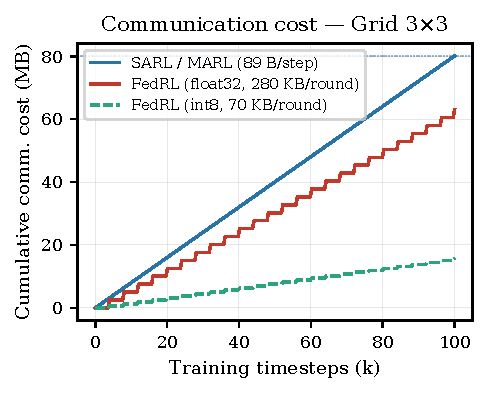
\includegraphics[width=\columnwidth]{fig_comm_cost.pdf}
\caption{Cumulative communication cost during training on Grid~3$\times$3. SARL/MARL stream 89~B/intersection/step continuously; FedRL exchanges $\approx$280~KB/intersection per aggregation round at float32 (or $\approx$70~KB under 8-bit post-training quantization). FedDistill, not plotted, sits at roughly 0.5~MB/round.}
\label{fig:comm}
\end{figure}

Raw performance is only half of the deployment story: the other half is what information must leave each roadside unit. This subsection analyzes communication cost only; the other two systems-level axes---training-time wall clock and per-step inference cost---are held constant by construction (same PPO recipe, same MLP architecture, same number of PPO epochs per round), so they do not differentiate strategies in a controlled comparison. Multi-strategy wall-clock and GPU-hour breakdowns on heterogeneous hardware are an orthogonal study that will accompany the extended HPC sweep (Section~\ref{sec:limits}). We analyze communication cost in three regimes.

\textbf{Continuous streaming (SARL, MARL).} Every timestep, each intersection sends (observation 56~B + action 1~B + V2I metadata 32~B) = 89~B to the central trainer. Over 100{,}000 steps this is 80.1~MB on Grid~3$\times$3 and 222.5~MB on Grid~5$\times$5.

\textbf{Periodic weight aggregation (FedRL).} Weights are exchanged once per 4000-step round. At float32, $\approx$280~KB per intersection per round $\times$ 25 rounds totals 129.0~MB of weight traffic on Grid~3$\times$3 (157.8~MB when combined with baseline telemetry)---nearly double SARL. With 8-bit post-training quantization (4$\times$ reduction), weight exchanges fall to 32.3~MB, bringing total FedRL cost to 61.1~MB, \textbf{24\% less than SARL}. The break-even quantization ratio is close to 4$\times$ on both grid sizes.

\textbf{Logit sharing (FedDistill).} Only action probabilities on a small shared observation bank are shared; per round this is on the order of 0.5~MB per intersection, or roughly 100$\times$ less than FedRL weights. FedDistill sits 3rd on Grid~3$\times$3 at the baseline demand (13.18~s), so the bandwidth saving is not free---but it is the most attractive performance-per-bit option in our set.

\textbf{Burstiness.} Beyond cumulative totals, FedRL and FedDistill traffic is \emph{bursty}---concentrated at round boundaries rather than streamed continuously. In bandwidth-constrained or intermittently-connected roadside deployments, this concentration pattern is often preferable to continuous streaming at the same total volume.

\section{Discussion}\label{sec:discussion}

\subsection{The Goldilocks Zone}
Stepping back from individual tables, the results point consistently to one observation: \emph{neither of the two extremes wins}. Fully-independent learning (MARL) leaves each intersection to rediscover the same patterns from scratch; no knowledge flows between agents, so training effort is duplicated and small intersections with thin traffic never see enough data. At the other extreme, fully-shared learning (SARL) ties all intersections to a single set of parameters and averages away the differences that matter on the ground---phase counts, neighbor geometry, and approach speeds. The winning strategies are the ones that share with \emph{road neighbors} but not with \emph{everyone}: Gossip (pairwise weight averaging with adjacent intersections) and HierFed (team-level weight averaging). These two sit in what we call the Goldilocks zone: enough common knowledge to coordinate, but still enough local specialization to fit local traffic.

\subsection{Interpreting the anomalies}
Three findings deserve explicit comment because each would look like noise in a less controlled study:
\begin{itemize}
\item \emph{CTDE's reversal.} CTDE is worst on Grid~3$\times$3 (15.29~s) and best on Grid~5$\times$5 (4.36~s). The centralized critic has variance that grows slowly with the number of agents, but its \emph{benefit} (coordinated value estimation) grows fast. On 9 intersections, the variance cost dominates; on 25, the coordination benefit dominates.
\item \emph{SARL at high demand on Grid~3$\times$3.} SARL is only 5th at baseline demand but wins at 600~VPLPH. At near-gridlock, the ``right'' action is almost always to advance the most overloaded phase, and a single shared policy learns this simple rule quickly. At moderate demand there is no such simple rule, and specialization matters more.
\item \emph{Cologne-8 shortfall.} All RL strategies are currently behind Fixed-Time on Cologne-8 at 50 episodes. This is a training-budget anomaly, not a coordination anomaly; the 200-episode HPC re-run in progress is expected to close the gap (see Section~\ref{sec:limits}).
\end{itemize}

\subsection{Deployment implications}
A practitioner choosing a strategy should consider three axes:
(i)~network size---small and uniform favors shared policies (SARL) or gentle sharing (Gossip); large and heterogeneous favors CTDE at training time and HierFed/Gossip at deployment;
(ii)~demand regime---light demand favors federation; heavy demand favors specialized or very-shared extremes;
(iii)~communication budget---if weight bandwidth is scarce, FedDistill buys most of the federation benefit at 1\% of the bits.

\section{Limitations and Future Work}\label{sec:limits}

\textbf{Single training seed, no formal significance tests.} The reported numbers use the baseline training seed~42 and 5 held-out evaluation seeds (42--46); a 270-run HPC variance sweep across 10 training seeds is in flight. 95\% bootstrap confidence intervals and Wilcoxon signed-rank significance tests (with Bonferroni correction for pairwise comparisons) are planned for the IEEE~ITSC submission once the variance sweep completes and are listed here as a gap rather than as reported results. We report point estimates only where the between-strategy gap is larger than the typical within-seed variance we have observed on completed runs.

\textbf{FedRL aggregation ablation not yet run.} The reward-weighted FedAvg variant in Eq.~\eqref{eq:rwfedavg} is described but not separately evaluated in this report. A direct ablation between plain FedAvg and the reward-weighted and FedProx variants is scheduled together with the HPC variance sweep; we avoided including unablated numbers to keep the controlled-comparison contract honest.

\textbf{Full-metric tables deferred.} This report uses waiting time as the headline metric; travel time, completed-trip counts, and throughput were computed and sanity-checked but their full per-cell tables are held for the journal extension to keep the present paper within the 10-page budget.

\textbf{Cologne-8 budget.} Thirty episodes is clearly insufficient for a real-world topology; the extended 200-episode campaign is the priority follow-up. Once complete, we will also report Ingolstadt-3 from RESCO.

\textbf{Metric horizon bias.} Average waiting time computed over \emph{completed} trips can favor aggressive policies that abandon queues on side streets (those vehicles never complete). We mitigate this by reporting completed-trip counts alongside; a fairness-aware metric (per-intersection worst-case waiting) is a natural next step.

\textbf{Simulation-only.} All results come from SUMO. Validation on CityFlow and VISSIM is planned, as is small-scale hardware-in-the-loop testing with real signal controllers.

\textbf{Algorithm axis.} We hold the RL algorithm at PPO throughout. Cross-algorithm comparisons (DQN, A2C, SAC) are a planned orthogonal sweep; the controlled-framework design makes this a drop-in extension.

\textbf{Larger networks.} A 7$\times$7 grid (49 intersections) and a full Cologne network (39 intersections) are on the HPC queue, targeting the question of whether the 25-intersection Goldilocks pattern persists at scale.

\section{Conclusion}\label{sec:conclusion}

We presented ATLAS, a standardized benchmark that isolates the training strategy as the sole independent variable for multi-intersection traffic signal control. Running ten strategies across synthetic and real-world topologies at three demand levels, we find that the best strategy depends on \emph{both} network size and demand regime, that strategies in a Goldilocks zone of road-neighbor sharing (Gossip, HierFed) are the most robust across conditions, and that federated logit sharing (FedDistill) offers a 100$\times$ communication reduction at a modest performance cost---a promising trade-off for bandwidth-constrained roadside deployments. The controlled-framework design reveals regime-dependent winners that single-setting studies miss and provides a reusable harness for future strategy comparisons.

Our planned extensions are directly enabled by the framework: new strategies plug into the trainer layer without touching the simulator, demand generator, observation pipeline, or evaluation harness. Adding an RL algorithm, a new topology, or a new aggregation recipe each takes a single file. We hope ATLAS lowers the barrier to fair, reproducible federated-RL research for traffic.

\section*{Acknowledgment}
The authors thank Mr.~Ahmed Sharshar for advising this project and the MBZUAI HPC team for compute access. Source code, trained weights, and the full evaluation harness are available at \url{https://github.com/HamdanKAlmehairbi/RoadsidePrediction}.

\begin{thebibliography}{00}
\bibitem{inrix2019} INRIX, ``INRIX 2019 global traffic scorecard,'' INRIX Research, 2019.
\bibitem{wei2020survey} H. Wei, G. Zheng, V. Gayah, and Z. Li, ``Recent advances in reinforcement learning for traffic signal control: a survey of models and evaluation,'' \textit{ACM SIGKDD Explorations Newsletter}, vol. 22, no. 2, pp. 12--18, 2020.
\bibitem{ault2021resco} J. Ault and G. Sharon, ``Reinforcement learning benchmarks for traffic signal control,'' in \textit{Proc. NeurIPS Datasets and Benchmarks Track}, 2021.
\bibitem{mei2024libsignal} H. Mei \textit{et al.}, ``LibSignal: an open library for traffic signal control,'' \textit{Machine Learning}, vol. 113, pp. 4619--4647, 2024.
\bibitem{ye2021fedlight} J. Ye, W. Zhao, J. Ye, and X. Song, ``FedLight: federated reinforcement learning for autonomous multi-intersection traffic signal control,'' in \textit{Proc. 58th ACM/IEEE Design Automation Conf. (DAC)}, 2021, pp. 847--852.
\bibitem{hudson2022seal} N. Hudson, J. Ault, and G. Sharon, ``SEAL: spatially-aware multi-agent reinforcement learning for traffic signal control,'' in \textit{Proc. IEEE SMARTCOMP}, 2022.
\bibitem{bao2023partial} Q. Bao, Y. Cao, and J. Wu, ``A scalable approach to optimize traffic signal control with federated reinforcement learning,'' \textit{Scientific Reports}, vol. 13, art. 18350, 2023.
\bibitem{fu2025hierfed} Z. Fu, Y. Shen, Y. Zhou, and X. Wang, ``Federated hierarchical reinforcement learning for adaptive traffic signal control,'' arXiv preprint arXiv:2504.05553, 2025.
\bibitem{mcmahan2017fedavg} B. McMahan, E. Moore, D. Ramage, S. Hampson, and B. A. y~Arcas, ``Communication-efficient learning of deep networks from decentralized data,'' in \textit{Proc. AISTATS}, 2017, pp. 1273--1282.
\bibitem{li2020fedprox} T. Li, A. K. Sahu, M. Zaheer, M. Sanjabi, A. Talwalkar, and V. Smith, ``Federated optimization in heterogeneous networks,'' in \textit{Proc. MLSys}, 2020.
\bibitem{jeong2018feddistill} E. Jeong, S. Oh, H. Kim, J. Park, M. Bennis, and S.-L. Kim, ``Communication-efficient on-device machine learning: federated distillation and augmentation under non-IID private data,'' in \textit{NeurIPS Machine Learning on the Phone Workshop}, 2018.
\bibitem{yang2018meanfield} Y. Yang, R. Luo, M. Li, M. Zhou, W. Zhang, and J. Wang, ``Mean field multi-agent reinforcement learning,'' in \textit{Proc. ICML}, 2018, pp. 5571--5580.
\bibitem{lowe2017maddpg} R. Lowe, Y. Wu, A. Tamar, J. Harb, P. Abbeel, and I. Mordatch, ``Multi-agent actor-critic for mixed cooperative-competitive environments,'' in \textit{Proc. NeurIPS}, 2017, pp. 6379--6390.
\bibitem{koloskova2020gossip} A. Koloskova, N. Loizou, S. Boreiri, M. Jaggi, and S. U. Stich, ``A unified theory of decentralized SGD with changing topology and local updates,'' in \textit{Proc. ICML}, 2020, pp. 5381--5393.
\bibitem{varaiya2013maxpressure} P. Varaiya, ``Max pressure control of a network of signalized intersections,'' \textit{Transportation Research Part C: Emerging Technologies}, vol. 36, pp. 177--195, 2013.
\bibitem{wei2019presslight} H. Wei \textit{et al.}, ``PressLight: learning max pressure control to coordinate traffic signals in arterial networks,'' in \textit{Proc. KDD}, 2019, pp. 1290--1298.
\bibitem{wei2019colight} H. Wei \textit{et al.}, ``CoLight: learning network-level cooperation for traffic signal control,'' in \textit{Proc. CIKM}, 2019, pp. 1913--1922.
\bibitem{schulman2017ppo} J. Schulman, F. Wolski, P. Dhariwal, A. Radford, and O. Klimov, ``Proximal policy optimization algorithms,'' arXiv preprint arXiv:1707.06347, 2017.
\bibitem{liang2018rllib} E. Liang \textit{et al.}, ``RLlib: abstractions for distributed reinforcement learning,'' in \textit{Proc. ICML}, 2018, pp. 3053--3062.
\bibitem{lopez2018sumo} P. A. Lopez \textit{et al.}, ``Microscopic traffic simulation using SUMO,'' in \textit{Proc. IEEE ITSC}, 2018, pp. 2575--2582.
\end{thebibliography}

\end{document}
